\documentclass{article}
\usepackage{amsmath}
\usepackage{graphicx}
\begin{document}
\title{Products: Question 17}
\author{Ana Bhattacharjee}
\date{\today}
\maketitle{}

\begin{center}
The first step is to find the ratio of the sides from square EFGH to E"F"G"H".
\begin{align}
H" (-9, -6), G" (-3, -6), E" (-9, -12), F" (-3, -12) \\
E (-6, 3), F (-2, 3), H (-6, -1), G (-2, -1) \\
EF = \sqrt{(-2 + 6)^2 + (3 - 3)^2} = 4 \\
E"F" = \sqrt{(-3 + 9)^2 - (-12 + 12)^2} = 6 \\
k = \frac{6}{4} = \frac{3}{2} \\
\end{align}
The next step is to use the reciprocol of the scale factor $(k^{-1})$ and multiply this reciprocol to each coordinate of the final transformation. The rationale for this is to find out the placement of E'F'G'H' before it was dilated.
\begin{align}
H' (\frac{2}{3}(-9, -6)) \rightarrow (-6, -4) \\
G' (\frac{2}{3}(-3, -6)) \rightarrow (-2, -4 ) \\
E' (\frac{2}{3}(-9, -12)) \rightarrow (-6, -8) \\
F' (\frac{2}{3}(-3, -12)) \rightarrow (-2, -8)
\end{align}
From these coordinates, a visualization of the square can immediately demonstrate that it has been vertically translated 3 units down from the original square EFGH. See the image below.
\begin{figure}[!htbp]
  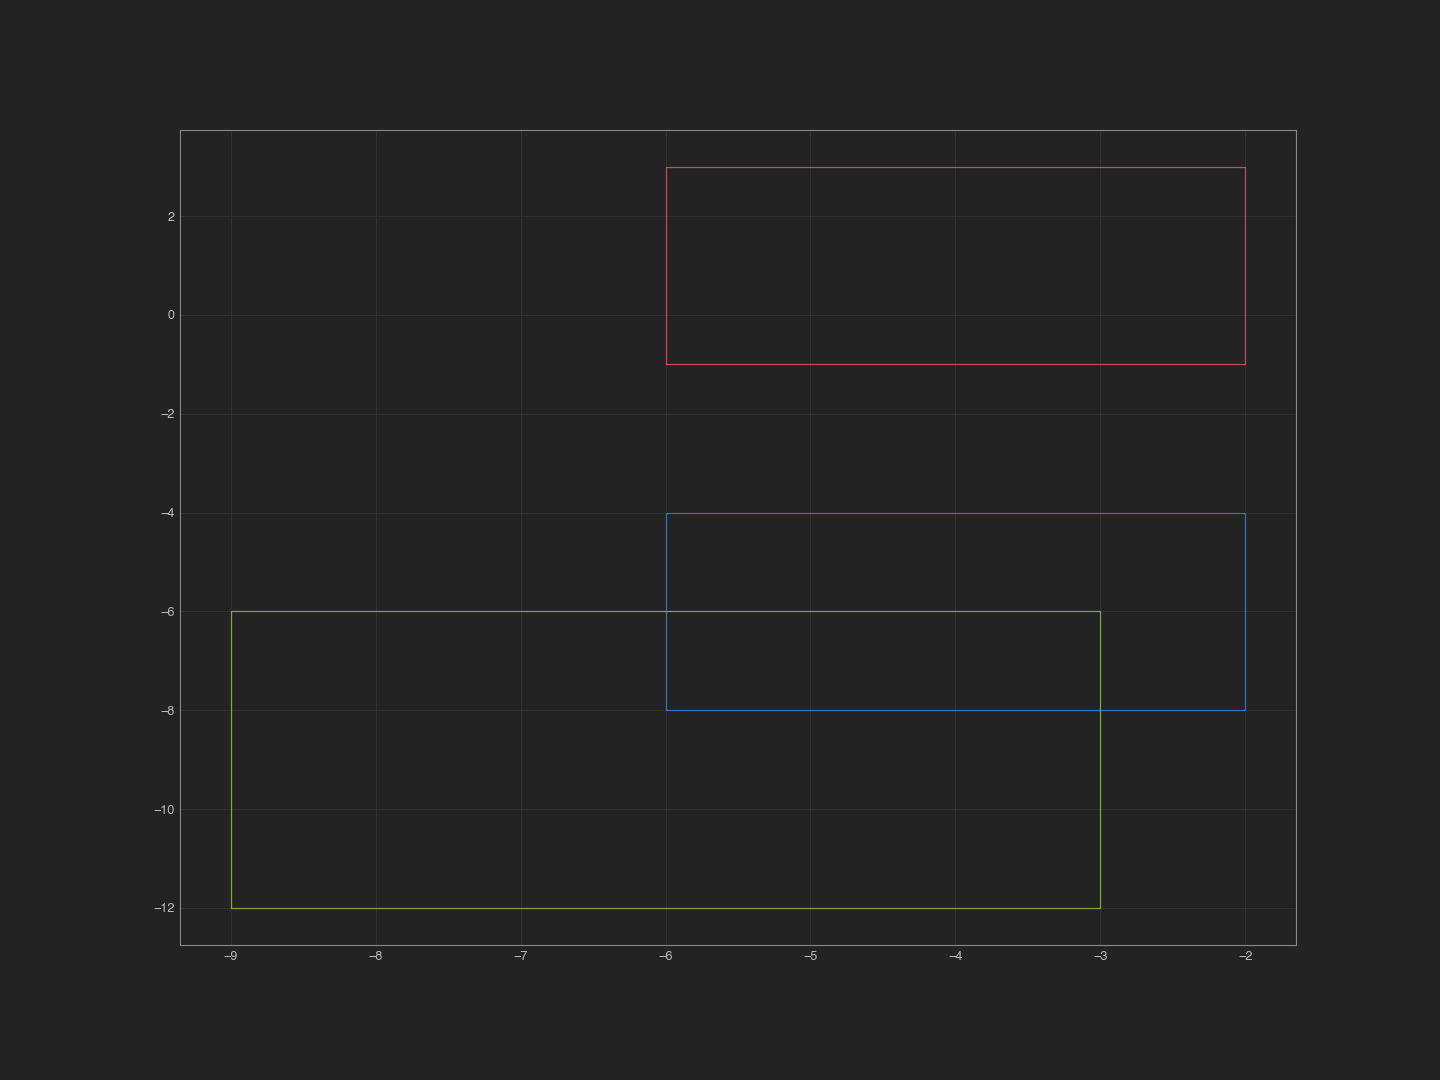
\includegraphics[width=1.0\columnwidth]{../q_17}
  \caption{Series of Transformations of EFGH (Red)}
\end{figure}
\end{center}
\end{document}
